%==============================================================================
% tento soubor pouzijte jako zaklad
% this file should be used as a base for the thesis
% Autoři / Authors: 2008 Michal Bidlo, 2016 Jaroslav Dytrych
% Kontakt pro dotazy a připomínky: dytrych@fit.vutbr.cz
% Contact for questions and comments: dytrych@fit.vutbr.cz
%==============================================================================
% kodovani: UTF-8 (zmena prikazem iconv, recode nebo cstocs)
% encoding: UTF-8 (you can change it by command iconv, recode or cstocs)
%------------------------------------------------------------------------------
% zpracování / processing: make, make pdf, make clean
%==============================================================================
% Soubory, které je nutné upravit: / Files which have to be edited:
%   projekt-20-literatura-bibliography.bib - literatura / bibliography
%   projekt-01-kapitoly-chapters.tex - obsah práce / the thesis content
%   projekt-30-prilohy-appendices.tex - přílohy / appendices
%==============================================================================
%\documentclass[]{fitthesis} % bez zadání - pro začátek práce, aby nebyl problém s překladem
%\documentclass[english]{fitthesis} % without assignment - for the work start to avoid compilation problem
%\documentclass[zadani]{fitthesis} % odevzdani do wisu - odkazy jsou barevné
%\documentclass[english,zadani]{fitthesis} % for submission to the IS FIT - links are color
%\documentclass[zadani,print]{fitthesis} % pro tisk - odkazy jsou černé
%\documentclass[zadani,cprint]{fitthesis} % pro barevný tisk - odkazy jsou černé, znak VUT barevný
%\documentclass[english,zadani,print]{fitthesis} % for the color print - links are black
%\documentclass[english,zadani,cprint]{fitthesis} % for the print - links are black, logo is color
% * Je-li práce psaná v anglickém jazyce, je zapotřebí u třídy použít
%   parametr english následovně:
%   If thesis is written in english, it is necessary to use 
%   parameter english as follows:
%      \documentclass[english]{fitthesis}
% * Je-li práce psaná ve slovenském jazyce, je zapotřebí u třídy použít
%   parametr slovak následovně:
%   If the work is written in the Slovak language, it is necessary
%   to use parameter slovak as follows:
%      \documentclass[slovak]{fitthesis}
% * Je-li práce psaná v anglickém jazyce se slovenským abstraktem apod.,
%   je zapotřebí u třídy použít parametry english a enslovak následovně:
%   If the work is written in English with the Slovak abstract, etc.,
%   it is necessary to use parameters english and enslovak as follows:
      \documentclass[english,enslovak]{fitthesis}

% Základní balíčky jsou dole v souboru šablony fitthesis.cls
% Basic packages are at the bottom of template file fitthesis.cls
% zde můžeme vložit vlastní balíčky / you can place own packages here
\usepackage{epigraph}
\usepackage{graphicx}
% Kompilace po částech (rychlejší, ale v náhledu nemusí být vše aktuální)
% Compilation piecewise (faster, but not all parts in preview will be up-to-date)
\usepackage{subfiles}

% Nastavení cesty k obrázkům
% Setting of a path to the pictures
%\graphicspath{{obrazky-figures/}{./obrazky-figures/}}
\graphicspath{{figures/}{../figures/}}

%---rm---------------
\renewcommand{\rmdefault}{lmr}%zavede Latin Modern Roman jako rm / set Latin Modern Roman as rm
%---sf---------------
\renewcommand{\sfdefault}{qhv}%zavede TeX Gyre Heros jako sf
%---tt------------
\renewcommand{\ttdefault}{lmtt}% zavede Latin Modern tt jako tt

% vypne funkci šablony, která automaticky nahrazuje uvozovky,
% aby nebyly prováděny nevhodné náhrady v popisech API apod.
% disables function of the template which replaces quotation marks
% to avoid unnecessary replacements in the API descriptions etc.
\csdoublequotesoff

% =======================================================================
% balíček "hyperref" vytváří klikací odkazy v pdf, pokud tedy použijeme pdflatex
% problém je, že balíček hyperref musí být uveden jako poslední, takže nemůže
% být v šabloně
% "hyperref" package create clickable links in pdf if you are using pdflatex.
% Problem is that this package have to be introduced as the last one so it 
% can not be placed in the template file.
\ifWis
\ifx\pdfoutput\undefined % nejedeme pod pdflatexem / we are not using pdflatex
\else
  \usepackage{color}
  \usepackage[unicode,colorlinks,hyperindex,plainpages=false,pdftex]{hyperref}
  \definecolor{links}{rgb}{0.4,0.5,0}
  \definecolor{anchors}{rgb}{1,0,0}
  \def\AnchorColor{anchors}
  \def\LinkColor{links}
  \def\pdfBorderAttrs{/Border [0 0 0] }  % bez okrajů kolem odkazů / without margins around links
  \pdfcompresslevel=9
\fi
\else % pro tisk budou odkazy, na které se dá klikat, černé / for the print clickable links will be black
\ifx\pdfoutput\undefined % nejedeme pod pdflatexem / we are not using pdflatex
\else
  \usepackage{color}
  \usepackage[unicode,colorlinks,hyperindex,plainpages=false,pdftex,urlcolor=black,linkcolor=black,citecolor=black]{hyperref}
  \definecolor{links}{rgb}{0,0,0}
  \definecolor{anchors}{rgb}{0,0,0}
  \def\AnchorColor{anchors}
  \def\LinkColor{links}
  \def\pdfBorderAttrs{/Border [0 0 0] } % bez okrajů kolem odkazů / without margins around links
  \pdfcompresslevel=9
\fi
\fi
% Řešení problému, kdy klikací odkazy na obrázky vedou za obrázek
% This solves the problems with links which leads after the picture
\usepackage[all]{hypcap}

% Informace o práci/projektu / Information about the thesis
%---------------------------------------------------------------------------
\projectinfo{
  %Prace / Thesis
  project={BP},            %typ práce BP/SP/DP/DR  / thesis type (SP = term project)
  year={2018},             % rok odevzdání / year of submission
  date=\today,             % datum odevzdání / submission date
  %Nazev prace / thesis title
  title.cs={Portovanie Tang na OpenWRT},  % název práce v češtině či slovenštině (dle zadání) / thesis title in czech language (according to assignment)
  title.en={Porting Tang to OpenWRT}, % název práce v angličtině / thesis title in english
  %title.length={14.5cm}, % nastavení délky bloku s titulkem pro úpravu zalomení řádku (lze definovat zde nebo níže) / setting the length of a block with a thesis title for adjusting a line break (can be defined here or below)
  %Autor / Author
  author.name={Tibor},   % jméno autora / author name
  author.surname={Dudlák},   % příjmení autora / author surname
  %author.title.p={Bc.}, % titul před jménem (nepovinné) / title before the name (optional)
  %author.title.a={Ph.D.}, % titul za jménem (nepovinné) / title after the name (optional)
  %Ustav / Department
  department={UPGM}, % doplňte příslušnou zkratku dle ústavu na zadání: UPSY/UIFS/UITS/UPGM / fill in appropriate abbreviation of the department according to assignment: UPSY/UIFS/UITS/UPGM
  % Školitel / supervisor
  supervisor.name={Ondrej},   % jméno školitele / supervisor name
  supervisor.surname={Lichtner},   % příjmení školitele / supervisor surname
  supervisor.title.p={Ing.},   %titul před jménem (nepovinné) / title before the name (optional)
  %supervisor.title.a={Ph.D.},    %titul za jménem (nepovinné) / title after the name (optional)
  % Klíčová slova / keywords
  %keywords.cs={Sem budou zapsána jednotlivá klíčová slova v českém (slovenském) jazyce, oddělená čárkami.}, % klíčová slova v českém či slovenském jazyce / keywords in czech or slovak language
  keywords.cs={portovanie, Tang, server, OpenWrt, operačný systém, vstavaný, Clevis, klient, Escrow, šifrovanie, LUKS,
 pevný disk, diskový oddiel, šifrovací kľúč, automatizácia, cross-kompilácia, balíkový systém }
  keywords.en={Sem budou zapsána jednotlivá klíčová slova v anglickém jazyce, oddělená čárkami.}, % klíčová slova v anglickém jazyce / keywords in english
  % Abstrakt / Abstract
  %abstract.cs={Do tohoto odstavce bude zapsán výtah (abstrakt) práce v českém (slovenském) jazyce.}, % abstrakt v českém či slovenském jazyce / abstract in czech or slovak language
  %abstract.en={Do tohoto odstavce bude zapsán výtah (abstrakt) práce v anglickém jazyce.}, % abstrakt v anglickém jazyce / abstract in english
  abstract.cs={Hlavným cieľom tejto práce je sprístupnenie serveru Tang na vstavané zariadenia typu WiFi smerovač s plne modulárnym operačným systémom OpenWrt. Tým dosiahneme anonymnú správu šifrovacích kľúčov pre domáce siete a siete malých firiem. Preto táto práca popisuje problematiku šifrovania a jeho využitie na zabezpečenie pevného disku počítača. Oboznámuje čitateľa so štruktúrou šifrovaného diskového oddielu podľa LUKS špecifikácie na operačných systémoch typu Linux. Práca rozoberá možnosti automatizácie odomykania šifrovaných diskov použitím externého servera, ktorý vstupuje do procesu ako tretia strana. Sú v nej popísané princípy serverov Key Escrow a Tang. Dosiahnutie hlavného cieľa je možné vďaka procesu portovania a cross-kompilácie na platforme Linux.  Práca obsahuje zdokumentovaný postup prispievania zmien a novo vytvorených balíkov pre OpenWrt do príslušných Open Source projektov.}
abstract.en={This thesis describes the encryption and its application to secure the computer's hard drive. It describes the structure of the encrypted disk's partition according to the LUKS specification on Linux operating systems. The thesis focus on describing possibilities of automating the disk decryption process using an external server that enters the process as a third party. It describes the principles of Key Escrow and Tang server. Steps required to compile and configure the Tang server are described too. Also described is Tang server's client -- Clevis. The main objective of this work was to port and document the process of porting the Tang server and its dependencies to OpenWrt system, described in this thesis too, which is designed for embedded devices such as WiFi routers. The thesis also includes a documented process of contributing changes and newly created OpenWrt packages to relevant Open Source projects.}
  % Prohlášení (u anglicky psané práce anglicky, u slovensky psané práce slovensky) / Declaration (for thesis in english should be in english)
  declaration={Hereby I declare that this term project was prepared as an original author’s work under the supervision of Ing. Ondrej Lichtner.
  The supplementary information was provided by Jan Pazdziora, Ph. D.
  All the relevant information sources, which were used during preparation of this thesis, are properly cited and included in the list of references.
  }
%declaration={Prohlašuji, že jsem tuto bakalářskou práci vypracoval samostatně pod vedením pana X...
%Další informace mi poskytli...
%Uvedl jsem všechny literární prameny a publikace, ze kterých jsem čerpal.},
  %declaration={Hereby I declare that this bachelor's thesis was prepared as an original author’s work under the supervision of Mr. X
% The supplementary information was provided by Mr. Y
% All the relevant information sources, which were used during preparation of this thesis, are properly cited and included in the list of references.},
  % Poděkování (nepovinné, nejlépe v jazyce práce) / Acknowledgement (optional, ideally in the language of the thesis)
  acknowledgment={V této sekci je možno uvést poděkování vedoucímu práce a těm, kteří poskytli odbornou pomoc
(externí zadavatel, konzultant, apod.).},
  %acknowledgment={Here it is possible to express thanks to the supervisor and to the people which provided professional help
%(external submitter, consultant, etc.).},
  % Rozšířený abstrakt (cca 3 normostrany) - lze definovat zde nebo níže / Extended abstract (approximately 3 standard pages) - can be defined here or below
  %extendedabstract={Do tohoto odstavce bude zapsán rozšířený výtah (abstrakt) práce v českém (slovenském) jazyce.},
  %faculty={FIT}, % FIT/FEKT/FSI/FA/FCH/FP/FAST/FAVU/USI/DEF
  faculty.cs={Fakulta informačních technologií}, % Fakulta v češtině - pro využití této položky výše zvolte fakultu DEF / Faculty in Czech - for use of this entry select DEF above
  faculty.en={Faculty of Information Technology}, % Fakulta v angličtině - pro využití této položky výše zvolte fakultu DEF / Faculty in English - for use of this entry select DEF above
  department.cs={Ústav matematiky}, % Ústav v češtině - pro využití této položky výše zvolte ústav DEF nebo jej zakomentujte / Department in Czech - for use of this entry select DEF above or comment it out
  department.en={Institute of Mathematics} % Ústav v angličtině - pro využití této položky výše zvolte ústav DEF nebo jej zakomentujte / Department in English - for use of this entry select DEF above or comment it out
}

% Rozšířený abstrakt (cca 3 normostrany) - lze definovat zde nebo výše / Extended abstract (approximately 3 standard pages) - can be defined here or above
%\extendedabstract{Do tohoto odstavce bude zapsán výtah (abstrakt) práce v českém (slovenském) jazyce.}

% nastavení délky bloku s titulkem pro úpravu zalomení řádku - lze definovat zde nebo výše / setting the length of a block with a thesis title for adjusting a line break - can be defined here or above
%\titlelength{14.5cm}


% řeší první/poslední řádek odstavce na předchozí/následující stránce
% solves first/last row of the paragraph on the previous/next page
\clubpenalty=10000
\widowpenalty=10000

\begin{document}
  % Vysazeni titulnich stran / Typesetting of the title pages
  % ----------------------------------------------
  \maketitle
  % Obsah
  % ----------------------------------------------
  \setlength{\parskip}{0pt}

  {\hypersetup{hidelinks}\tableofcontents}
  
  % Seznam obrazku a tabulek (pokud prace obsahuje velke mnozstvi obrazku, tak se to hodi)
  % List of figures and list of tables (if the thesis contains a lot of pictures, it is good)
  \ifczech
    \renewcommand\listfigurename{Seznam obrázků}
  \fi
  \ifslovak
    \renewcommand\listfigurename{Zoznam obrázkov}
  \fi
  % \listoffigures

  \ifczech
    \renewcommand\listtablename{Seznam tabulek}
  \fi
  \ifslovak
    \renewcommand\listtablename{Zoznam tabuliek}
  \fi
  % \listoftables

  \ifODSAZ
    \setlength{\parskip}{0.5\bigskipamount}
  \else
    \setlength{\parskip}{0pt}
  \fi

  % vynechani stranky v oboustrannem rezimu
  % Skip the page in the two-sided mode
  \iftwoside
    \cleardoublepage
  \fi

  % Text prace / Thesis text
  % ----------------------------------------------
  \documentclass[../xdudla00-porting-Tang-to-Open-WRT.tex]{subfiles}
\begin{document}
%=========================================================================
% (c) Michal Bidlo, Bohuslav Křena, 2008

\chapter{Introduction}\label{introduction}

Nowadays, the whole world uses information technologies to communicate and simply to spread knowledge in form of bits to the other people.  But there are personal information such as photos from a family vacation, videos of our children as they grow, contracts, testaments and so on which we would like to protect.

Encryption protects our data even when we do not know that. It protects our conversation privacy, personal information stored all over governmental authorities, bank accounts, in general data transmitted around the internet and stored on our hard drives. Encryption provides process of transforming our information in such way that only trusted person can decrypt data and access it. An unauthorized person might be able to access secured data but will not be able to read the information from them without the proper key. The most important thing is keeping the encryption key (the password) a secret.

The goal of this bachelor thesis will be to port % https://en.wikipedia.org/wiki/Porting
{\it Tang} server \ref{tang}, its dependencies, and {\it Clevis} framework \ref{clevis} to {\it OpenWRT} system \ref{owrt}. With accomplishing, this we will be able to automatize process of unlocking encrypted drives on our private respectively home network. There will be no need for any decryption server but only {\it OpenWRT} device running the {\it Tang} server itself.

%My primary goal is to focus on the packaging system of the {\it OpenWRT} and build processes on it.\todo{Treba to doplnit...}

%($\backslash${\tt cite\{identifikator\}}).


\end{document}

  \documentclass[../xdudla00-porting-Tang-to-Open-WRT.tex]{subfiles}
\begin{document}

\chapter{Encryption}\label{encryption}

For most of us is common to have a password protected system.
But the encrypted disk requires another password (key) to decrypt.
Imagine that you came home in mood to enjoy your time and your system ask for password not once but twice.
I think this is reason why most of us do not use encryption even when we know it will protect our data.
This is what Tang \ref{tang} is for and to whom is for because we want automatize things.

Lets look how the encryption is typically done. As you can see in the image below it all starts with desire to keep our data to ourselves and as a secret to the other people.
At the most these secrets are stored on our hard drives. Usually we encrypt this secret by using an encryption key.
But our secret data might grow in size, and it is time and resource consuming to decrypt and encrypt secret every time encryption key changes or it is compromised.
Because of that we wrap encrypted data in the key encryption key and this is what system prompts from us on boot.
So changing key encryption key does not affect encrypted data and we can change it whenever we desire to.

\begin{figure}[h]
    \centering
    
\includegraphics{../figures/placeholder.pdf}
    \caption{How we encrypt data}
    \label{fig:encdata}
\end{figure}

\todo{dopisat}

\end{document}
  \documentclass[../xdudla00-porting-Tang-to-Open-WRT.tex]{subfiles}
\begin{document}

\chapter{Escrow}\label{escrow}
Before Tang, automated decryption was handled usually with key escrow.
Client using key escrow usually generates a key, encrypt data with it and then stores the key in a remote server.
Key escrow server (also known as a “fair” cryptosystem) stores decryption keys. This should signal potential security risks when storing and also transmitting keys over network.
For security purposes key escrow uses SSL/TLS to provide privacy and data integrity between server and client.
Even with SSL/TLS key escrow requires authentication.
\todo{Treba to doplnit...}
To sum up an authorized third party may gain access to those keys under certain circumstances only.

\end{document}

  %\documentclass[../xdudla00-porting-Tang-to-Open-WRT.tex]{subfiles}

%\begin{document}

\chapter{Tang server}\label{tang} \todo{re-factor entire chapter}
Tang server is an open source project implemented in C programming language, and it binds data to network presence.
What does binding data to network presence really mean?
Essentially, it allows us to make some data to be available only when the system containing the data is on a particular, usually secure, network.

\section{Tang - binding daemon}

Tang server advertises asymmetric keys and a client is able to get the list of these signing keys \ref{jose} by HTTP (Hypertext Transfer Protocol) GET request.
The next step is the provisioning step. With the list of these public keys the process of encrypting data may start.
A client chooses one of the asymmetric keys to generate a unique encryption key.
After this, the client encrypts data using the created key. Once the data is encrypted, the key is discarded.
Some small metadata have to be produced as a part of this operation. The client should store these metadata to work with it when decrypting.

Finally, when the client wants to access the encrypted data, it must be able to recover encryption key.
This step starts with loading the stored metadata and ends with simply performing a HTTP POST to Tang server.
Server performs its mathematical operation and sends the result back to the client.
Finally, the client has to calculate the key value, which is better than when server calculates it.
So the Tang server never knew the value of the key and literraly nothing about its clients.

\begin{figure}[h]
    \centering
    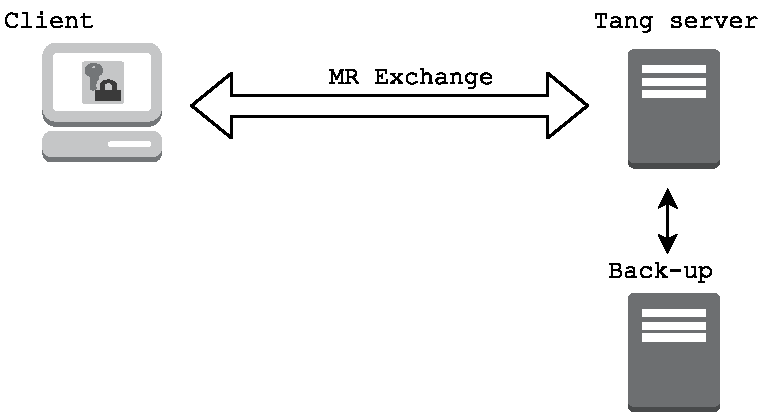
\includegraphics[scale=0.7]{figures/TangModel.pdf}
    \caption{Tang model}
    \label{fig:tangmodel}
\end{figure}

On Figure \ref{fig:tangmodel} you can see the Tang model.
It is very similar to Escrow model \ref{fig:escrowmodel} but there are some thing missing.
In fact, there is no longer a need for TLS channel to secure comunication between the client and the server,
 and that is the reason why Tang implements the McCallum-Relyea exchange \ref{mrexchange} as described below.

\section{Binding with Tang}

A client performs an ECDH key exchange using the McCallum-Relyea algorithm \ref{mrexchange} in order to generate the binding key.
Then the client discards its own private key so that the Tang server is the only party that can reconstitute the binding key.
To blind \todo{blind?} the client's public key and the binding key, Tang uses a third, ephemeral key.
Ephemeral key is generated for each execution of a key establishment process.
Now only the client can unblind his public key and binding key.
\todo{ARROWS}
\begin{table}[h]
\centering
\label{mrexchange}
\begin{tabular}{c|c|c|c}
\hline
\multicolumn{2}{c|}{Provisioning} & \multicolumn{2}{c}{Recovery} \\ \hline  used
client's side & server's side & client's side & server's side \\ \hline
 & $ S \epsilon _{R} [1, p-1]$ & $E \epsilon _{R} [1, p-1]$ &  \\
 & $s = gS$ &$ x = c + gE$ &  \\
 & $\leftarrow$  s &  x $\rightarrow$ &  \\
$C \epsilon _{R} [1, p-1]$ &  &  & $y = zS $\\
$e = gC $&  &  & $\leftarrow$ y \\
$K = gSC = sC$ &  & $K = y - sE $&  \\
Discard: K, C &  &  &  \\
Retain s, c &  &  &  \\ \hline
\end{tabular}
\caption{McCallum-Relyea exchange}
\end{table}

\section{Provisioning}
The client selects one of the Tang server's exchange keys (we will call it sJWK; identified by the use of deriveKey in the sJWK's key\_ops attribute).
The lowercase "s" stands for server's key pair and JWK is used format of the message.
The client generates a new (random) JWK (cJWK; c stands for client's key pair).
The client performs its half of a standard ECDH exchange producing dJWK which it uses to encrypt the data.
Afterwards, it discards dJWK and the private key from cJWK.

The client then stores cJWK for later use in the recovery step.
Generally speaking, the client may also store other data, such as the URL of the Tang server or the trusted advertisement signing keys.

\begin{equation}
    s = g * S
\end{equation}

\begin{equation}
    c = g * C
\end{equation}

\begin{equation}
    K = s * C
\end{equation}

\section{Recovery}
To recover dJWK after discarding it, the client generates a third ephemeral key (eJWK).
Using eJWK, the client performs elliptic curve group addition of eJWK and cJWK, producing xJWK. The client POSTs xJWK to the server.

The server then performs its half of the ECDH key exchange using xJWK and sJWK, producing yJWK. The server returns yJWK to the client.

The client then performs half of an ECDH key exchange between eJWK and sJWK, producing zJWK. Subtracing zJWK from yJWK produces dJWK again.

Mathematically (capital is private key; g stands for generate) client's operation:

\begin{equation}
    e = g * E
\end{equation}

\begin{equation}
    x = c + e
\end{equation}

\begin{equation}
    y = x * S
\end{equation}

\begin{equation}
    z = s * E
\end{equation}

\begin{equation}
    K = y - z
\end{equation}

\section{Security}

We can now compare Tang and Escrow. In contrast, Tang is stateless and doesn't require TLS or authentication.
Tang also has limited knowledge. Unlike escrows, where the server has knowledge of every key ever used, Tang never sees a single client key.
Tang never gains any identifying information from the client.

\begin{table}[h]
\centering
\label{compare}
\begin{tabular}{@{}lll@{}}
\toprule
               & Escrow   & Tang                         \\ \midrule
Stateless      & No       & Yes                          \\
SSL/TLS        & Required & Optional                     \\
X.509          & Required & Optional                     \\
Authentication & Required & Optional                     \\
Anonymous      & No       & Yes                          \\ \bottomrule
\end{tabular}
\caption{Comparing Escrow and Tang}
\end{table}

Let's think about the security of Tang system. Is it really secure without an encrypted channel or even without authentication?
So long as the client discards its private key, the client cannot recover dJWK without the Tang server.
This is fundamentally the same assumption used by Diffie-Hellman (and ECDH).

\subsection{Man-in-the-Middle attack}
In this case, the eavesdropper in this case sees the client send xJWK and receive yJWK.
Since, these packets are blinded by eJWK, only the party that can unblind these values is the client itself (since only it has eJWK's private key).
Thus, the MitM attack fails.
\subsection{Compromise the client to gain access to cJWK}
It is of utmost importance that the client protects cJWK from prying eyes.
This may include device permissions, filesystem permissions, security frameworks (such as SELinux - Security-Enhanced Linux) or even the use of hardware encryption such as a TPM.
How precisely this is accomplished depends on the client implementation.
\subsection{Compromise the server to gain access to sJWK's private key}
The Tang server must protect the private key for sJWK.
In this implementation, access is controlled by file system permissions and the service's policy.
An alternative implementation might use hardware cryptography (for example, an HSM) to protect the private key.
\section{Building Tang}

Tang is originally packaged for Fedora OS version 23 and later but we can build it from source of course.
It relies on few other software libraries:
\label{dependencies}
\begin{itemize}
\item http-parser \ref{http-parser}
\item systemd / xinetd \ref{systemd}
\item jose \ref{jose}
    \begin{itemize}
    \item jansson \ref{jansson}
    \item openssl \ref{openssl}
    \item zlib \ref{zlib}
    \end{itemize}
\end{itemize}

The steps to build it from source include download source from poject's GitHub or clone~it.
Make sure you have all needed dependencies installed and then run:

{\tt \$ autoreconf -if}

{\tt \$ ./configure --prefix=/usr}

{\tt \$ make}

{\tt \$ sudo make install}

Optionally to run tests:

{\tt \$ make check}

\subsection{http-parser}\label{http-parser}
Tang uses this parser for both parsing HTTP requests and HTTP responses.
The parser can be found on its own GitHub \cite{http-parser}.

\subsection{systemd / xinetd}\label{systemd}
systemd is a suite of basic building blocks for a Linux system.
It provides a system and service manager that runs as PID 1 and starts the rest of the system.
systemd provides aggressive parallelization capabilities, uses socket and D-Bus activation for starting services,
 offers on-demand starting of daemons, keeps track of processes using Linux control groups, maintains mount and automount points,
 and implements an elaborate transactional dependency-based service control logic.
\todo{Why is systemd needed by tang}

\subsection{José}\label{jose}
José \cite{jose_prog} is a C-language implementation of the Javascript Object Signing and Encryption standards.
Specifically, José aims towards implementing the following standards:
\begin{itemize}
   \item RFC 7515 - JSON Web Signature (JWS)        \cite{JWS}
   \item RFC 7516 - JSON Web Encryption (JWE)       \cite{JWE}
   \item RFC 7517 - JSON Web Key (JWK)              \cite{JWK}
   \item RFC 7518 - JSON Web Algorithms (JWA)       \cite{JWA}
   \item RFC 7519 - JSON Web Token (JWT)            \cite{JWT}
   \item RFC 7520 - Examples of ... JOSE            %\cite{RFC7520}
   \item RFC 7638 - JSON Web Key (JWK) Thumbprint   \cite{JWK}
\end{itemize}

JOSE (Javascript Object Signing and Encryption) is a framework intended to provide a method to securely transfer claims (such as authorization information) between parties.

Tang uses JWKs in comunication between client and server. Both POST request and reply bodies are JWK objects.

\subsection{jansson}\label{jansson}
Jansson \cite{jansson}(licenced under MIT licence) is a C library for encoding, decoding and manipulating JSON data. It features:
\begin{itemize}

    \item Simple and intuitive API and data model
    \item Comprehensive documentation
    \item No dependencies on other libraries
    \item Full Unicode support (UTF-8)
    \item Extensive test suite
\end{itemize}

\subsection{OpenSSL}\label{openssl}
OpenSSL contains an open-source implementation of the Transport Layer Security (TLS) and Secure Sockets Layer (SSL) protocols.
It is used by network applications to secure communication between two parties over network.

\subsection{zlib}\label{zlib}
Library zlib \cite{zlib} is used for data compression.

\section{Server enablement}
Enabling a Tang server is a two-step process.
First, enable and start the service using systemd.

{\tt\begin{verbatim} $ sudo systemctl enable tangd-update.path\end{verbatim}
}

{\tt\begin{verbatim} $ sudo systemctl start tangd-update.path\end{verbatim}
}

{\tt\begin{verbatim} $ sudo systemctl enable tangd.socket\end{verbatim}
}

{\tt\begin{verbatim} $ sudo systemctl start tangd.socket\end{verbatim}
}

Second, generate a signing key and an exchange key.

{\tt\begin{verbatim} $ sudo jose gen -t '{"alg":"ES256"}' -o /var/db/tang/sig.jwk\end{verbatim}
}

{\tt\begin{verbatim} $ sudo jose gen -t '{"kty":"EC","crv":"P-256","key_ops":["deriveKey"]}' \
        -o /var/db/tang/exc.jwk\end{verbatim}
}

Now we are up and running. Server is ready to send advertisment on demand.
\todo{Get clevis in here?}


\section{Clevis client}\label{clevis}

Clevis provides a pluggable key management framework for automated decryption.
It can handle even automated unlocking of LUKS volumes.
To do so, we have to encrypt some data with simple command:

{\tt\begin{verbatim} $ clevis encrypt PIN CONFIG < PLAINTEXT > CIPHERTEXT.jwe\end{verbatim}
}

In clevis terminology, a {\it pin} is a plugin which implements automated decryption.
We simply pass the name of supported pin here.
Secondly {\it config} is a JSON object which will be passed directly to the {\it pin}.
It contains all the necessary configuration to perform encryption and setup automated decryption.

\subsection{PIN: Tang}
Clevis has full support for Tang. Here is an example of how to use Clevis with Tang:
{\tt \begin{verbatim} $ echo hi | clevis encrypt tang '{"url": "http://tangserver"}' > hi.jwe
 The advertisement is signed with the following keys:
     kWwirxc5PhkFIH0yE28nc-EvjDY

 Do you wish to trust the advertisement? [yN] y\end{verbatim}
}
In this example, we encrypt the message "hi" using the Tang pin.
The only parameter needed in this case is the URL of the Tang server.
During the encryption process, the Tang pin requests the key advertisement from the server and asks you to trust the keys.
This works similarly to SSH.

Alternatively, you can manually load the advertisment using the adv parameter.
This parameter takes either a string referencing the file where the advertisement is stored, or the JSON contents of the advertisment itself.
When the advertisment is specified manually like this, Clevis presumes that the advertisement is trusted.
\subsection{PIN: HTTP}
Clevis also ships a pin for performing escrow using HTTP.
Please note that, at this time, this pin does not provide HTTPS support and is suitable only for use over local sockets.
This provides integration with services like Custodia.

\subsection{PIN: SSS - Shamir Secret Sharing}
Clevis provides a way to mix pins together to provide sophisticated unlocking policies.
This is accomplished by using an algorithm called Shamir Secret Sharing (SSS).

\subsection{Binding LUKS volumes}
Clevis can be used to bind a LUKS volume using a pin so that it can be automatically unlocked.

How this works is rather simple. We generate a new, cryptographically strong key. This key is added to LUKS as an additional passphrase. We then encrypt this key using Clevis, and store the output JWE inside the LUKS header using LUKSMeta.

Here is an example where we bind {\tt /dev/vda2} using the Tang ping:
{\tt \begin{verbatim} $ sudo clevis bind-luks /dev/sda1 tang '{"url": "http://tang.local"}'
 The advertisement is signed with the following keys:
         kWwirxc5PhkFIH0yE28nc-EvjDY

 Do you wish to trust the advertisement? [yN] y
 Enter existing LUKS password:\end{verbatim}
}
Upon successful completion of this binding process, the disk can be unlocked using one of the provided unlockers.

\subsection{Dracut}\label{dracut}
The Dracut unlocker attempts to automatically unlock volumes during early boot.
This permits automated root volume encryption.
Just rebuild your initramfs after installing Clevis:

{\tt \begin{verbatim} $ sudo dracut -f\end{verbatim}
}

Upon reboot, you will be prompted to unlock the volume using a password. In the background, Clevis will attempt to unlock the volume automatically. If it succeeds, the password prompt will be cancelled and boot will continue.

\subsection{UDisks2}\label{udisk2}
Our UDisks2 unlocker runs in your desktop session.
You should not need to manually enable it; just install the Clevis UDisks2 unlocker and restart your desktop session.
The unlocker should be started automatically.

This unlocker works almost exactly the same as the Dracut unlocker.
If you insert a removable storage device that has been bound with Clevis, we will attempt to unlock it automatically in parallel with a desktop password prompt.
If automatic unlocking succeeds, the password prompt will be dissmissed without user intervention.


%\end{document}

  \documentclass[../xdudla00-porting-Tang-to-Open-WRT.tex]{subfiles}
\begin{document}

\chapter{OpenWrt system}\label{owrt}
OpenWrt is a Linux distribution for embedded devices especially for wireless routers.
It was originally developed in January 2004 for the Linksys WRT54G with buildroot from the uClibc project.
Now it supports many more models of routers. 
Installing OpenWrt system means replacing your router’s built-in firmware with the Linux system which provides a fully writable filesystem with package management. 
This means that we are not bound to applications provided by the vendor.
Router (the embedded device) with this distribution can be used for anything that an embedded Linux system can be used for, from using its SSH Server for SSH Tunneling, to running lightweight server software (e.g. IRC server) on it. 
In fact it allows us to customize the device through the use of packages to suit any application.

Today (May 2017) the stable 15.05.1 release of OpenWrt (code-named "Chaos Calmer") released in March 2016 using Linux kernel version 3.18.23 runs on many routers.

\section{OPKG Package manager}

The opkg utility (Open Package Management System) is a lightweight package manager used to download and install OpenWrt packages.
The opkg is fork of an ipkg (Itsy Package Management System).
These packages could be stored somewhere on device's filesystem or the package manager will download them from local package repositories or ones located on the Internet mirrors. 
Users already familiar with GNU/Linux package managers like apt/apt-get, pacman, yum, dnf, emerge etc. will definitely recognize the similarities.
It also has similarities with NSLU2's Optware, also made for embedded devices.
Fact that OPKG is also a full package manager for the root file system, instead of just a way to add software to a seperate directory (e.g. /opt) includes the possibility to add kernel modules and drivers.
OPKG is sometimes called Entware, but this is mainly to refer to the Entware repository for embedded devices.

Opkg attempts to resolve dependencies with packages in the repositories - if this fails, it will report an error, and abort the installation of that package.

Missing dependencies with third-party packages are probably available from the source of the package.

\subsection{OPKG Makefile}




\end{document}

  \chapter{Software portability}\label{porting}

Ideally, any software would be usable on any operating system, platform, and any processor architecture.
Existence of term "porting", derived from the Latin portāre which means "to~carry", proves that this ideal situation does not occurs that often, and acctual process of "carrying" software to system with different environment is most probably required.
Porting is also used to describe procces of converting computer games to became platform independent.

Software porting procces might be hard to distinguish with building software.
The reason might be that in many cases building software on desired platform is enough, when software application does not work "out of the box".
This kind of behavior, an application that works immediately after or even without any special installation and without need for any configuration or modification, is ideal.
It often happens when we copy application from one desktop computer to another one, not realizing that they have processors with same instructions set and same or very simmilar operating system.
But let us be realistic, it depends on many things, such as processor architecture to which was application written (compiled), quality of design, how application is meant to be deployed and of course application's source code.

Porting is process not documented and required if we want to run thing on another platform \cite{porting_software}

Number of significantly different central processor units (CPUs), and operating systems used on the desktop or server is much smaller than in the past. \todo{Architectures}
Embeded ARM MIPS  RISC CISC x8664

Nowadays, the goal should be to develop software which is portable between preferred computer platforms (Linux, UNIX, Apple, Microsoft).
If software is considered as not portable, it could not have to mean immediately that it is not possible, just that time and resources spent porting already written software are almost comparable, or even significantly higher than writing software as a whole from scratch.
Effort spent porting some software product to work on desired platform must be little, such as copying already installed files to usb flash drive and run it on another computer.
This kind of approach might most probably fail, due to not present dependencies of third party libraries not present on destination computer.
Despite dominance of the x86 architecture there is usually a need to recompile software running, not only on different operating systems, to make sure we have all the dependencies present.

To simplify portability, even on distinguished processors with distant instruction sets, modern compilers translate source code to a machine-independent intermediate code.
But still, in the embedded system market, where OpenWrt belongs to, porting remains a significant issue.

\section{Porting to OpenWrt} %http://www.lemis.com/grog/Documentation/PUS/porting_unix_software-complete.pdf

Porting to openwrt means crosscompiling software on our computer because OpenWrt was not meant to be built on.
There are many mirrors containg openwrt SDK buildroots but when developing upstream projet upstream build root might be best solution.
problems with SDKs on mirrors are that they are most likely outdated and dependencies required to make it possible to build on this SDK might be not possible to get on your platform

\subsection{upstream buildroot}

Upstream Buildroot of OpenWrt is on github back then patches could been submitted by mailing list
it contains openwrt root, packages root, we will see how they are connected and how to use them.
But first we need to install all the dependencies that we need for this buildroot to be functional and ready to produce packages for our desired architecture on OpenWrt platform
Dependencies can be found on openwrt forum but i will list used depences on my system fedora 27

list dependencies and their versions

version of upstream buildroot is as mentioned important i have been working with upstream and all changes on upstream may affect your buildroot and maybe need to update dependency for buildroots
latest working upsream master commit that we were working with is ADD

we can clone build root from upstream with git Worflow should be to fork, clone forked copy to ourselves set upstream origin then when creating or wanting to edit any package we should create branch for this changes and then commit patches to this branch
when branch is ready create pull request and hope for the best that it wont be automatically revoked and just minor changes will be required.
after comunication with upstream and resolving all the possible issues our patch is ready to push to upstream.

where upstream changes are? how i can download ltest packages and what should i do to have them on my system?

\subsection{working with buildroot}

describe buildroot topology and descibe what every single thing is what for
make will trigger making all packages not like in sdk
difference working with sdk and buildroot that sdk build only packages and buildroot can buld only package but it is designed to build entire image
for specified architecture respectively device from list
do not know how to add there new device but may provide link
configured with make menuconfig shown here firstly select architecture and configuration will be generated into .config :
in sdk .config is pre generated and make menuconfig (need to find out if possible)

on sdk make will trigger only buildinf packages in directory package and it has to be done right way
it is also possible to do this with build root but is better to have upstream or own packages there in right directory

screen

make menuconfig is to select all packages which we want to build  todo findout if it is neccessary to buld base packages for selected

make

feeds install -a

tm tmp is needed if package directory has been edited to regenerate metadata of what (todo find out)

it is better to know what we are installig with feeds install and to choose only required packages for one newly choosed package to build

\subsection{Makefiles}

This is very important part of creating new packages therefore porting them to openwrt this file is similar to specfiles on fedora and

  \documentclass[../xdudla00-porting-Tang-to-Open-WRT.tex]{subfiles}
\begin{document}

\chapter{Contributing}\label{contrib}

\todo{TODO chapter}

Z

\todo{mailing lists}

A

\todo{github}

\end{document}
  \chapter{Conclusion}\label{conlusion}



The Tang \ref{tang} server is a very lightweight program.
It provides secure and anonymous data binding using McCallum-Relyea exchange \ref{mrexchange} algorythm.

As every server purpose is to serve its clients, it needs to have client application.
In case of Tang we have Clevis.
Clevis \ref{clevis} is a client software with full support for Tang.
It has minimal dependencies and it is possible to use with HTTP, Escrow \ref{escrow}, and it implements Shamir Secret Sharing.
Clevis has GNOME integration so it is not only a command line tool.
Clevis also supports removable devices unocking using UDisks2 or even early boot integration with dracut, which was this thesis inspiration and goal to achieve with only embedded device supported OpenWrt running Tang server.

To port Tang to OpenWrt system it was necesarry to port all its dependencies first.
The OpenWrt system has already package openssl, zlib, and jansson but only version 2.7 which was too old.
So there was a need for updating jansson to resolve all dependencies for package José.
José required porting and after focusing on upstream version porting on this package was straightforward.
After struggling with older version, package http-parser known as libhttp-parser in OpenWrt feeds, is now updated to latest upstream version 2.8.0.
The systemd would be huge effort but tang's requirements are minimal and we were able to work with xinetd's socket activation.
With correct configuration of xinetd and removing dependency for systemd Tang server is running on OpenWrt with some platform specific changes mentioned in chapter \ref{porting-tang} Porting Tang.


  % Kompilace po částech (viz výše, nutno odkomentovat)
  % Compilation piecewise (see above, it is necessary to uncomment it)
  %\subfile{projekt-01-uvod-introduction}
  % ...
  \subfile{chapters/xdudla00-porting-Tang-to-Open-WRT-01-introduction}
  \subfile{chapters/xdudla00-porting-Tang-to-Open-WRT-02-encryption}
  \subfile{chapters/xdudla00-porting-Tang-to-Open-WRT-03-escrow}
  \subfile{chapters/xdudla00-porting-Tang-to-Open-WRT-04-tang}
  \subfile{chapters/xdudla00-porting-Tang-to-Open-WRT-05-openwrt}
  \subfile{chapters/xdudla00-porting-Tang-to-Open-WRT-06-porting}
  \subfile{chapters/xdudla00-porting-Tang-to-Open-WRT-07-contributing}
  \subfile{chapters/xdudla00-porting-Tang-to-Open-WRT-08-conclusion}

  % Pouzita literatura / Bibliography
  % ----------------------------------------------
\ifslovak
  \makeatletter
  \def\@openbib@code{\addcontentsline{toc}{chapter}{Literatúra}}
  \makeatother
  \bibliographystyle{bib-styles/czechiso}
\else
  \ifczech
    \makeatletter
    \def\@openbib@code{\addcontentsline{toc}{chapter}{Literatura}}
    \makeatother
    \bibliographystyle{bib-styles/czechiso}
  \else 
    \makeatletter
    \def\@openbib@code{\addcontentsline{toc}{chapter}{Bibliography}}
    \makeatother
    \bibliographystyle{bib-styles/englishiso}
  %  \bibliographystyle{alpha}
  \fi
\fi
  \begin{flushleft}
  \bibliography{bibl/xdudla00-porting-Tang-to-Open-WRT-20-bibliography,bibl/bibl_rfc_1-3826}
  \end{flushleft}

  % vynechani stranky v oboustrannem rezimu
  % Skip the page in the two-sided mode
  \iftwoside
    \cleardoublepage
  \fi

  % Prilohy / Appendices
  % ---------------------------------------------
  \appendix
\ifczech
  \renewcommand{\appendixpagename}{Přílohy}
  \renewcommand{\appendixtocname}{Přílohy}
  \renewcommand{\appendixname}{Příloha}
\fi
\ifslovak
  \renewcommand{\appendixpagename}{Prílohy}
  \renewcommand{\appendixtocname}{Prílohy}
  \renewcommand{\appendixname}{Príloha}
\fi
%  \appendixpage

% vynechani stranky v oboustrannem rezimu
% Skip the page in the two-sided mode
%\iftwoside
%  \cleardoublepage
%\fi

\ifslovak
%  \section*{Zoznam príloh}
%  \addcontentsline{toc}{section}{Zoznam príloh}
\else
  \ifczech
%    \section*{Seznam příloh}
%    \addcontentsline{toc}{section}{Seznam příloh}
  \else
%    \section*{List of Appendices}
%    \addcontentsline{toc}{section}{List of Appendices}
  \fi
\fi
  \startcontents[chapters]
  \setlength{\parskip}{0pt}
  % seznam příloh / list of appendices
  % \printcontents[chapters]{l}{0}{\setcounter{tocdepth}{2}}
  
  \ifODSAZ
    \setlength{\parskip}{0.5\bigskipamount}
  \else
    \setlength{\parskip}{0pt}
  \fi

  % vynechani stranky v oboustrannem rezimu
  \iftwoside
    \cleardoublepage
  \fi

  % Přílohy / Appendices
  % ----------------------------------------------
  \chapter{Disk content}

  \chapter{LUKS In-Place Encryption}
\label{luksipc}
It takes 4 steps to perform an in place encryption with {\it luksipc} \cite{luksipc}:
\begin{enumerate}
    \item Unmounting the filesystem
    \item Resizing the filesystem to shrink about 10 megabytes (2048 kB is the current LUKS header size -- but do not trust this value, it has changed in the past!)
    \item Performing luksipc
    \item Adding custom keys to the LUKS keyring
\end{enumerate}

\section{Step 1 - unmounting}

There should not be any problems unmounting partition, unless you want to encrypt / - the root partition, which in our case (to lock whole disk) will be necessary.
To do so we need to restart our computer and boot any other or live distribution capable of completing these next steps.

{\tt \# umount /dev/vda2}

\section{Step 2 - resizing}

There are plenty tools for re-sizing, essentially for partitioning as whole (fdisk, e2fsck, etc.).
Demonstrating how this is done for ext 2, 3, 4 here:

{\tt \# e2fsck /dev/vda2}

{\tt \# resize2fs /dev/vda2 -s -10M}

Delete and recreate shrinked partition with fdisk:

{\tt \# fdisk /dev/vda
Welcome to fdisk (util-linux 2.23.2).

Changes will remain in memory only, until you decide to write them. Be careful before using the write command.

Command (m for help):}

Check the partition number:

{\tt Command (m for help): p
Disk /dev/vda: 407.6 GiB, 437629485056 bytes, 854745088 sectors
Units: sectors of 1 * 512 = 512 bytes
Sector size (logical/physical): 512 bytes / 4096 bytes
I/O size (minimum/optimal): 4096 bytes / 4096 bytes
Disklabel type: dos
Disk identifier: 0x5c873cba
Partition 2 does not start on physical sector boundary.

Device        Boot        Start     End         Blocks      Id    System
/dev/vda1      *          2048      1026047     512000      83    Linux
/dev/vda2                 1026048   1640447     307200      8e    Linux LVM}

\section{Step 3 - encrypting}
After this, luksipc comes into play. It performs an in-place encryption of the data and prepends the partition with a LUKS header. Firt we have to download luksipc or install it with package manager.

{\tt \$ wget https://github.com/johndoe31415/luksipc/archive/master.zip}

{\tt \$ unzip master.zip}

{\tt \$ cd luksipc-master/}

{\tt \$ make}

Now run it with parameters like:

{\tt \# ./luksipc -d /dev/vda2}

luksipc will have created a key file /root/initial\_keyfile.bin that you can use to gain access to the newly created LUKS device:

{\tt \# cryptsetup luksOpen --key-file /root/initial\_keyfile.bin /dev/vda2 fedoradrive}

\section{Step 4 - adding key}

DO NOT FORGET to add key to LUKS volume:

{\tt \# cryptsetup luksAddKey --key-file /root/initial\_keyfile.bin /dev/vda2}

  \chapter{LUKS In Place Encryption}
\label{luksipc}
It takes 4 steps to perform an in place encryption with {\it luksipc} :
\begin{enumerate}
    \item Unmounting the filesystem
    \item Resizing the filesystem to shrink about 10 megabytes (2048 kB is the current LUKS header size -- but do not trust this value, it has changed in the past!)
    \item Performing luksipc
    \item Adding custom keys to the LUKS keyring
\end{enumerate}

\section{Step 1 - unmounting}

There should not be any problems unmounting partition, unless you want to encrypt / - the root partition, which in our case (to lock whole disk) will be necessary.
To do so we need to restart our computer and boot any other or live distribution capable of completing these next steps.

{\tt \# umount /dev/vda2}

\section{Step 2 - resizing}

There are plenty tools for re-sizing, essentially for partitioning as whole (fdisk, e2fsck, etc.).
Demonstrating how this is done for ext 2, 3, 4 here:

{\tt \# e2fsck /dev/vda2}

{\tt \# resize2fs /dev/vda2 -s -10M}

Delete and recreate shrinked partition with fdisk:

{\tt \# fdisk /dev/vda
Welcome to fdisk (util-linux 2.23.2).

Changes will remain in memory only, until you decide to write them. Be careful before using the write command.

Command (m for help):}

Check the partition number:

{\tt Command (m for help): p
Disk /dev/vda: 407.6 GiB, 437629485056 bytes, 854745088 sectors
Units: sectors of 1 * 512 = 512 bytes
Sector size (logical/physical): 512 bytes / 4096 bytes
I/O size (minimum/optimal): 4096 bytes / 4096 bytes
Disklabel type: dos
Disk identifier: 0x5c873cba
Partition 2 does not start on physical sector boundary.

Device        Boot        Start     End         Blocks      Id    System
/dev/vda1      *          2048      1026047     512000      83    Linux
/dev/vda2                 1026048   1640447     307200      8e    Linux LVM}

\section{Step 3 - encrypting}
After this, luksipc comes into play. It performs an in-place encryption of the data and prepends the partition with a LUKS header. Firt we have to download luksipc or install it with package manager.

{\tt \$ wget https://github.com/johndoe31415/luksipc/archive/master.zip}

{\tt \$ unzip master.zip}

{\tt \$ cd luksipc-master/}

{\tt \$ make}

Now run it with parameters like:

{\tt \# ./luksipc -d /dev/vda2}

luksipc will have created a key file /root/initial\_keyfile.bin that you can use to gain access to the newly created LUKS device:

{\tt \# cryptsetup luksOpen --key-file /root/initial\_keyfile.bin /dev/vda2 fedoradrive}

\section{Step 4 - adding key}

DO NOT FORGET to add key to LUKS volume:

{\tt \# cryptsetup luksAddKey --key-file /root/initial\_keyfile.bin /dev/vda2}

  % ----------------------------------------------

  % kompilace po částech (viz výše, nutno odkomentovat)
  % compilation piecewise (see above, it is necessary to uncomment it)
  \subfile{chapters/xdudla00-porting-Tang-to-Open-WRT-30-appendix-A}
  \subfile{chapters/xdudla00-porting-Tang-to-Open-WRT-31-appendix-B}
  \subfile{chapters/xdudla00-porting-Tang-to-Open-WRT-32-appendix-C}

\end{document}
